% #############################################################################
% This is Chapter 4
% !TEX root = ../main.tex
% #############################################################################
% Change the Name of the Chapter i the following line
\fancychapter{Evaluation}
%\cleardoublepage
\label{chap:evaluation}
 
This chapter focuses on the evaluation of the proposed framework from two perspectives: in \cref{sec:qualitative}, we discuss the qualitative properties of the optimization framework, outlining the flexibility and heterogeneity of the provided algorithms, while in \Cref{sec:quantitative}, we assess the viability of the current prototype in the architectural practice by applying it to address three \ac{BPO} case studies. These optimization case studies corroborate the suitability of the algorithmic framework described in \cref{chap:implement}, by using the optimization framework and the Khepri \ac{AD} tool to enable the application of different optimization algorithms. 

Overall, this evaluation aims to answer the following questions: 
\begin{itemize}
	\item Do the studied algorithms present benefits for the architectural practice? Particularly, are they able to reduce the impact of the expensive performance analysis that are typically employed in building design?
	\item Is there any algorithm or class of algorithms that constantly outperforms others?
	% \item Is there any difference between the different \ac{MOO} approaches? \todo{PAPER ACADIA}
	\item Is the proposed framework applicable to the architectural practice? 
\end{itemize}

\section{Qualitative Evaluation}
\todo{REVER}
\label{sec:qualitative}
The quantitative evaluation of optimization frameworks involve considering multiple aspects, including the flexibility, adaptability, diversity of algorithms, ease of use, among others. Calling upon the \acp{NFLT} discussed in \Cref{ssec:comparisondfo}, some algorithms are really good solvers for some problems and very poor solvers for others~\cite{Wolpert1997NFLT}. Selecting the right algorithm can have a great impact in the efficiency of optimization processes. Particularly, in building design, to benefit from such performance gains, diversity of algorithms allows to face each problems' characteristics differently, enabling the identification of most promising algorithms. In addition to the algorithms' diversity, algorithms should be effortlessly run, without the need for many manual changes, in order to be easily used by less experienced users. Notwithstanding their innate simplicity, optimization frameworks should also be flexible enough to enable more experienced users to fine-tune them according to their expertise, thus fostering more efficient optimization processes. At last, a good framework should adapt to handle different problems.

Regarding the adaptability of the current implementation of the framework, it provides mechanisms to address both single- and multi-objective problems: 15 \ac{SOO} algorithms and 13 \acp{MOEA}, respectively. Simpler approaches, like the design of experiments approach, discussed in \cref{ssec:doe}, are also possible using one of the 5 sampling methods available in the prototype. Moreover, a crucial feature of this framework is that it provides 10 \ac{ML} algorithms to be used with other techniques, thus allowing to reduce the time complexity involved in building design. 

In \cref{chap:architecture}, \cref{table:algorithms} presents a view of the algorithms supported by the framework, discriminated by class and domain. When comparing to currently existing tools in architecture, our solution presents a more extense and diverse set of algorithms, which can be explored to address a wider variety of problems. Moreover, while the existing tools rely on a unique optimization approach (e.g., \ac{SOO}, or Pareto-based optimization), our solution adapts to the user needs, providing the necessary mechanisms to the different approaches.

Unlike existing tools, which are implemented on top of visual programming languages, like Grasshopper and Dynamo, the framework is currently implemented on top of a textual programming language. Although the graphical feel of the visual paradigm provides a more comfortable experience to less experienced users, the fact that the framework makes use of the textual paradigm confers more scalability and portability to the achieved designs, thus allowing users to seamless apply optimization to more complex buildings. To make it more appealing to less experienced users, the developed optimization framework is in a ready-to-use format, where every parameter of an optimization process is configured by default.  

Besides the ready-to-use format, the framework supports finer configurations of the different algorithms, thus allowing more experienced users to employ their knowledge to fine-tune and, if desired, to combine different algorithms. 

Moreover, given the importance of testing different algorithms before settling for a single one~\cite{Wortmann2016BBO}, the prototype provides the necessary mechanisms to facilitate and automate testing multiple algorithms with no additional efforts for the user. Conversely, existing architectural tools require the user's intervention in order to test different algorithms, either by dragging other optimizer components and making necessary changes in the design script or, when possible, by simply re-configuring the optimization tool to use one of the other supported algorithms. 

Regarding the post-processing and logging mechanisms, the proposed framework is automatically configured to produce complete log files, including all the information about the algorithms and problems being addressed, as well as a real-time log of the different solutions explored during the optimization run. This differs from existing tools, which only made the log files available in the end of the run. That being said, some of the currently existing tools still outperform the proposed prototype in terms of the visualization and interactivity features. The proposed provides visual interactive Python scripts that read the log files and produce the corresponding plots. However, these plots are not updated in real-time, instead requiring the user to re-run the script.

Finally, in order to use the optimization framework, the user only needs to create the \ac{AD} and model the corresponding optimization problem, i.e., define the variables and its bounds, the objectives, and, if necessary, the constraints. In contrast to existing architectural optimization tools, which require the modification of the optimization script (e.g., drag other components, redefine the optimization problem, change the optimization tool), our framework requires no such effort. Instead, the user only needs to specify the algorithms that he wishes to apply and configure them accordingly.

% #############################################################################
\section{Quantitative Evaluation}
\label{sec:quantitative}

In order to study and explore the effectiveness of algorithms within building design practices, we evaluate the performance of different algorithms using the optimization framework, discussed in \cref{chap:implement}. Moreover, we evaluate the real applicability of such framework in three case studies, two of which were proposed by a small-scale architectural studio\footnote{Atelier dos Remédios: http://atrem.eu/}: (1) the optimization of the lighting conditions of a solarium in a private house in Portugal; (2) the optimization of the structural behavior and the elegance of an arc-shaped space frame structure; and (3) the optimization of the cost and the lighting conditions of an exhibition room in an arts pavilion.   

In order to measure the effectiveness of the optimization algorithms, different factors must be considered: (1) the optimization time is sensitive to the computational power of the machine where the algorithm is being run, (2) the non-determinism of several optimization algorithms, and (3) the hyperparameters of optimization algorithms. Firstly, to remove the time dependency of the machine and function's complexity, we measure the performance of the optimization algorithm in terms of the number of function evaluations, which is proportional to the actual time spent by the optimization process. Secondly, the stochastic character of several optimization algorithms (e.g., random modifications of solutions, random generation of design solutions, random initial points) might yield different results even when ran twice under the same configurations. To address this limitation, we run each stochastic algorithm 3 times and we use the average of the values to draw conclusions. Finally, the algorithm's performance for each problem can be better or worse depending on its configurations. To this end, we opt for using the default algorithm's configurations, thus emulating the case when architect's knowledge does not suffice to properly fine-tune the algorithm.
 
% #############################################################################
\subsection{Ericeira House: Solarium}
The first case study involves the optimization of the lighting conditions of a room in an isolated private house in Portugal~\cite{Caetano2018,Belem2018optimizeddesign}. The room was designed with a set of façade shading panels that modulate the daylight conditions on the interior of the room. Depicted in \cref{fig:ericeira_panels_explanation}, the panels are composed of a set of horizontal wood bars of different sizes, which alternate between one full-length bar and a set of smaller bars. For aesthetics reasons, the size and position of the smaller bars along the panel's width were randomized. The final pattern of the façade's shading panels is, thus, defined in function of four variables: the length’s step, the maximum distance separating two consecutive bars, and the minimum and maximum lengths of the smaller bars. Initially, the goal was to find a solution for the shading panels that maximized the room's daylight performance, which was measured using the \ac{sUDI} metric~\cite{Nabil2006}. In general, it is known that the more openings in the shading panels, the more daylight will enter the room. However, this may also cause situations of uncomfortable glare and therefore, which must be be accounted for. Moreover, taking into account aesthetics, the architects initially imposed a few constraints on the variables to reflect their intention for more dense patterns, i.e., with less openings. \Cref{fig:ericeira_multiple_panels} represents some design variations, ranging from denser patterns, with lower \ac{sUDI} values, to sparser ones, with higher \ac{sUDI} values.

\begin{figure}[htbp]
	\centering
	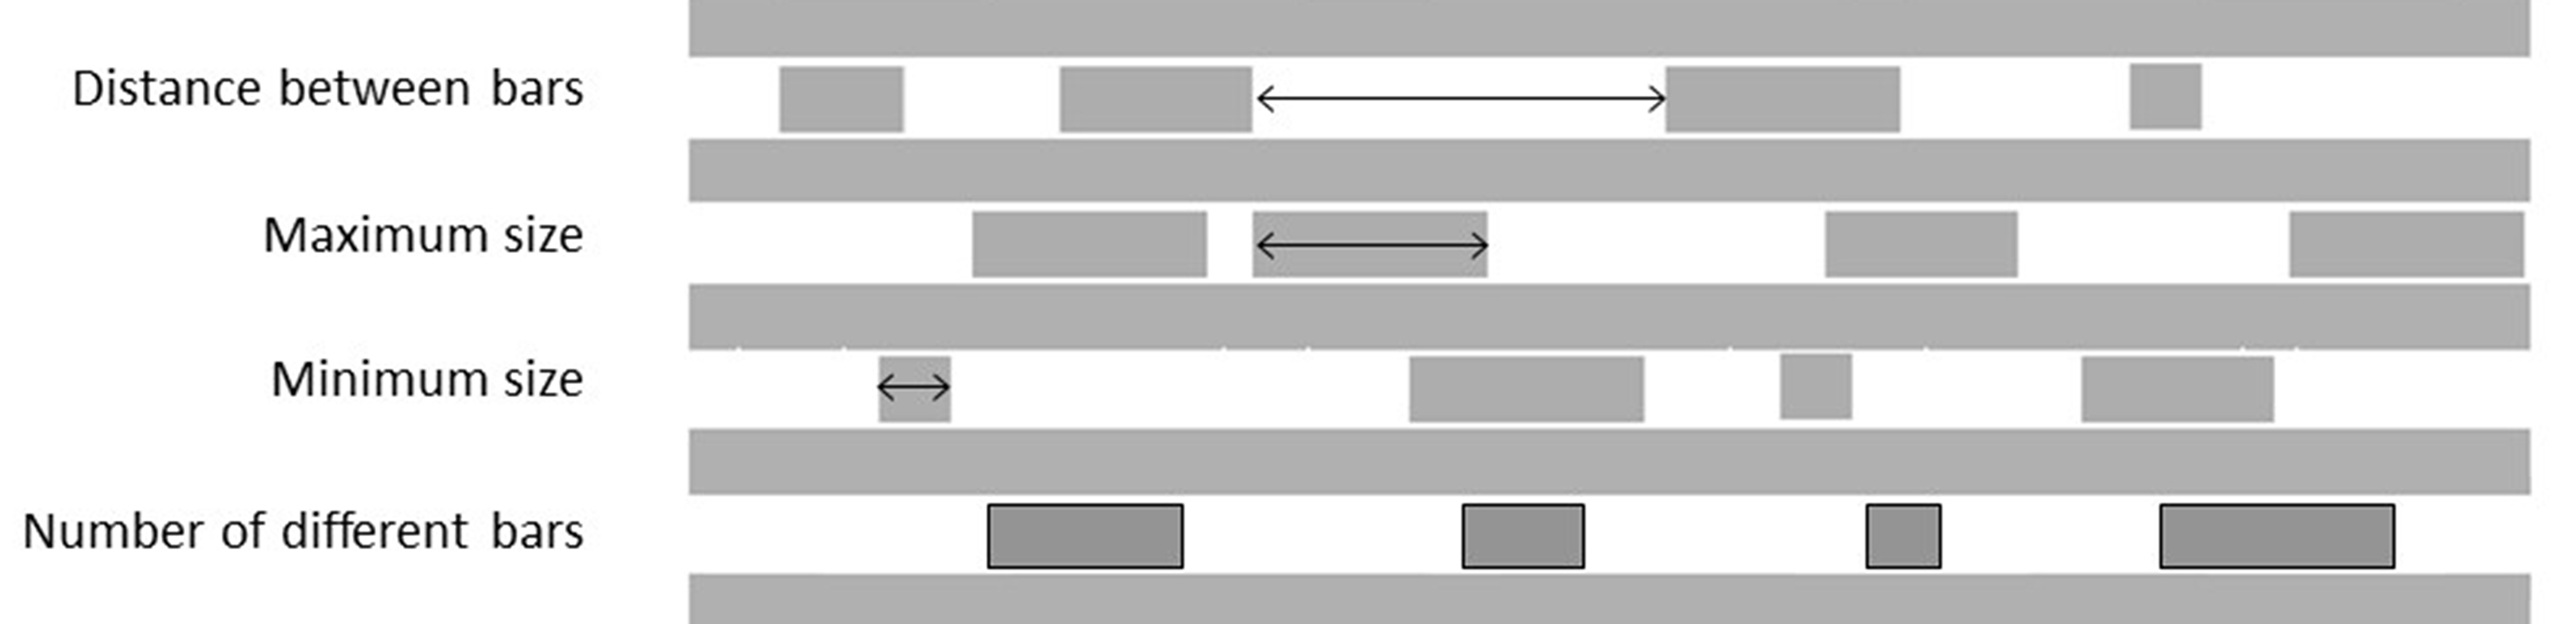
\includegraphics[width=\textwidth]{Images/Evaluation/Ericeira_1.jpg}
	\caption{Ericeira Solarium: Representation of the shading panels' geometric pattern and the patterns' design variables.}
	\label{fig:ericeira_panels_explanation}
\end{figure}

Our first approach to this case study was to a simple design of experiments \cite{Caetano2018}, where we used two sampling algorithms to generate different design approaches: the Monte Carlo sampling and the Latin hypercube sampling algorithms (see \cref{appendix:AlgorithmsDefinitions}). This approach allowed us to exploit the knowledge about the problem to produce a more efficient optimization process, by incrementally narrowing down the variables' bounds and, hence, enforcing the sampling of more efficient designs. %\Cref{fig:ericeira_doe} shows an example of the results obtained during this process, as well as the solutions that were presented to the architects, so that they would choose the one that better suited their intentions.

%\begin{figure}[htbp]
%	\centering
%	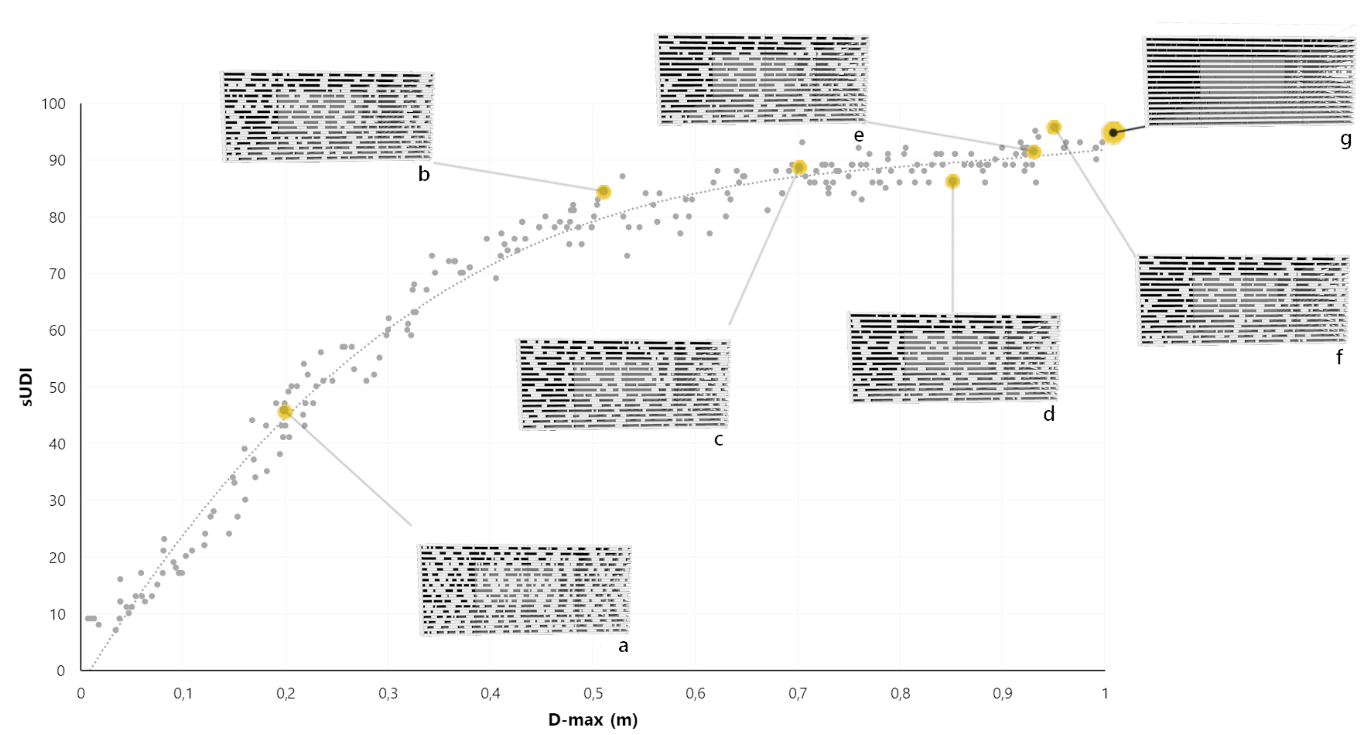
\includegraphics[width=\textwidth]{Images/Evaluation/Ericeira_caadria2018.PNG}
%	\caption{Ericeira Solarium: The scatter plot with the samples obtained during the design of experiments approach. The models a. to g. correspond to the set of examples presented to the architects.}
%	\label{fig:ericeira_doe}
%\end{figure}

\begin{figure}
	\centering
	\includegraphics[width=\textwidth]{Images/Evaluation/Ericeira_2.png}
	\caption{Ericeira Solarium: Representation of the shading panels’ geometric pattern with different sUDI values (from left to right, 7\%, 62\%, 90\%, and 100\%).}
	\label{fig:ericeira_multiple_panels}
\end{figure}

Although this approach did achieve an optimal solution with an 100\% value of sUDI after 200 function evaluations, this approach consists on the consecutive experimentation of multiple designs that are generated randomly and, consequently, does not provide guarantees that optimal solutions will be found. In this case study, we exploited the existing knowledge about the problem to create a more focused design of experiments approach, however it required several manual interventions (e.g., analyse the results, redefine the variables' bounds, select number of evaluations). As a result, we decided to use a more informed and automated approach \cite{Belem2018optimizeddesign}. Because this was a single-objective problem, we followed a simple \ac{SOO} approach (see \cref{ssec:soo}) and we evaluated the performance of 13 different derivative-free optimization algorithms: 5 direct-search, 3 metaheuristics, and 5 model-based. Given the time complexity of each function evaluation, we set a limit of 60 function evaluations per run.

\Cref{table:phase1results} shows the mean best results and the standard deviation of the three runs,  discriminated by algorithm. According to the results, in average, all global model-based algorithms, GPR, RBFCC, and RBFCL, were able to find an optimal solution within the first 30 evaluations of the optimization run. Conversely, the local model-based algorithms, COBYLA and BOBYQA, perform rather poorly in this problem, converging to far from optimal solutions after 29 and 48 function evaluations, respectively. Regarding direct-search algorithms, the global algorithm, DIRECT, was able to find a close to optimal solution (with an \ac{sUDI} value of 98\%) in the last function evaluation. While its local variant, DIRECT-L, and others local direct-search algorithms, PRAXIS and SUBPLEX, fell short of the expected and barely managed to improve over the 80\%. Nevertheless, a simplex-based direct-search algorithm, NMS, performed surprisingly well, having achieved an average result of 89.67\% within the first 15 function evaluations. Finally, although metaheuristics performed better than most local model-based and direct-search algorithms, they seem to stagnate in design solutions with sUDI values below the 88\%, after 30 function evaluations.

%http://papers.cumincad.org/data/works/att/caadria2018\_278.pdf
\begin{table}[htbp]
	\centering
	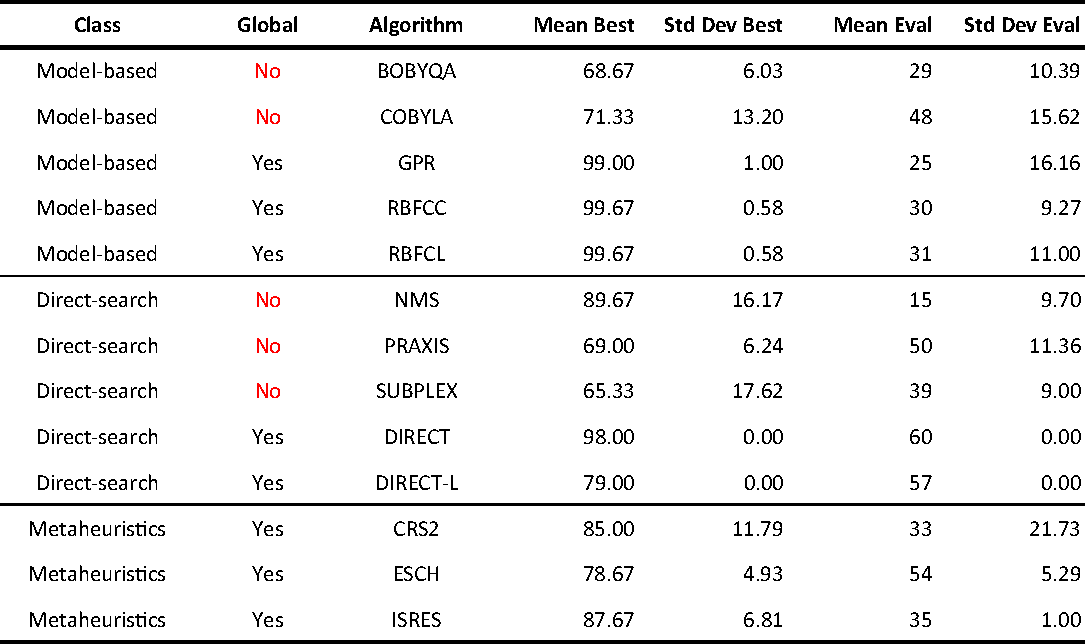
\includegraphics[width=0.8\textwidth]{tables_and_code/Ericeira_phase1_stats_v1.pdf}
	\caption[Ericeira Solarium: Table with best results and necessary evaluations per algorithm]{Ericeira Solarium: Table with the best results of daylight conditions (measured in \ac{sUDI}) per algorithm. Results are averaged over 3 runs, each with 60 evaluations. The table also depicts the average number of necessary evaluations to achieve best results.}
	\label{table:phase1results}
\end{table}

\Cref{fig:phase1results} shows the average performance per algorithm class, also separating them in local or global algorithms. Overall, local algorithms seem to perform worse than all other algorithms, with local direct-search and model-based algorithms stagnating towards design solutions with sUDI values below 75\% and 70\%, respectively. Contrastingly, global algorithms were able to find design solutions with values of sUDI larger than 80\%. Despite the better initial performance of metaheuristics for the first 20 evaluations, global direct-search methods quickly surpassed them, achieving close to optimal solutions with \ac{sUDI} values of 90\%. Global model-based algorithms were the best performing algorithms. 

\begin{figure}[htbp]
	\centering
	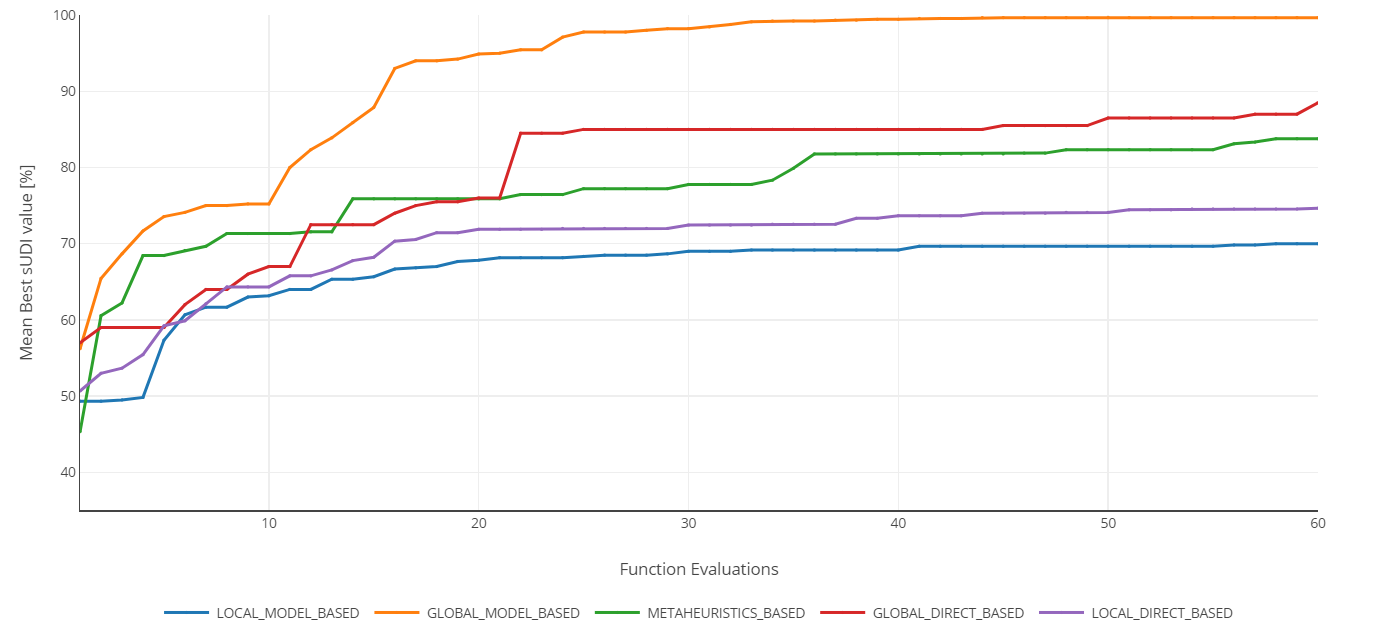
\includegraphics[width=1\textwidth]{Images/Evaluation/Ericeira_results_ph1_per_class.PNG}
	\caption[Ericeira Solarium: Average best results of daylight conditions (measured in \ac{sUDI}) per algorithm's class]{Ericeira Solarium: Average best results of daylight conditions (measured in \ac{sUDI}) per algorithm, as a function of the number of evaluations.}
	\label{fig:phase1results}
\end{figure}

Given the bad performance of local algorithms, we decided to assess their performance when submitted to different initial solutions. Notwithstanding their ability to quickly converge to locally optimal solutions, the quality of the found solutions highly depends on the initial one. To assess the impact of the initial solution in the performance of the algorithms, we submitted them to two different solutions: a bad one with a 7\% value of \ac{sUDI}, and a mild one with a 78\% value of \ac{sUDI}. Moreover, we decided to further constrain the number of function evaluations to 15, thus emulating an ideal scenario, where users lack knowledge about different optimization algorithms, and, as a consequence, opt for testing several algorithms. Ideally, this test would allow them to infer the most promising algorithm and obtain a reasonable solution to hot-start other algorithms and, potentially, improve the overall optimization time.

\Cref{fig:phase2results} presents the mean best daylight conditions found by each local optimization algorithm. As expected no local algorithm was able to obtain a good solution when provided with a bad starting solution. On the one hand, when provided with a mild initial design, both COBYLA and NMS found the best designs achieving a \ac{sUDI} value of 99\%. On the contrary, PRAXIS found the worse, and showed no relevant improvement over the initial design in terms of daylight illuminance. Nevertheless, it initially managed to outperform other methods, achieving values of \ac{sUDI} of 80\%. After the eighth evaluation, COBYLA and NMS quickly converged to near optimal designs, with \ac{sUDI} values of 99\% and 98\%, respectively. BOBYQA and SUBPLEX struggled to improve from the initial design.

On the other hand, when provided with a bad initial design, the best daylight illuminance result has a \ac{sUDI} value of 15\% and was found by NMS after the ninth evaluation. NMS, COBYLA, and SUBPLEX exhibit similar performances, stagnating in a design with a \ac{sUDI} value of 11\% after 3 evaluations, with NMS being able to further improve the design after 5 evaluations. PRAXIS exhibits the worst performance among all methods, showing no significant improvements throughout the whole optimization process.

\begin{figure}[htbp]
	\centering
	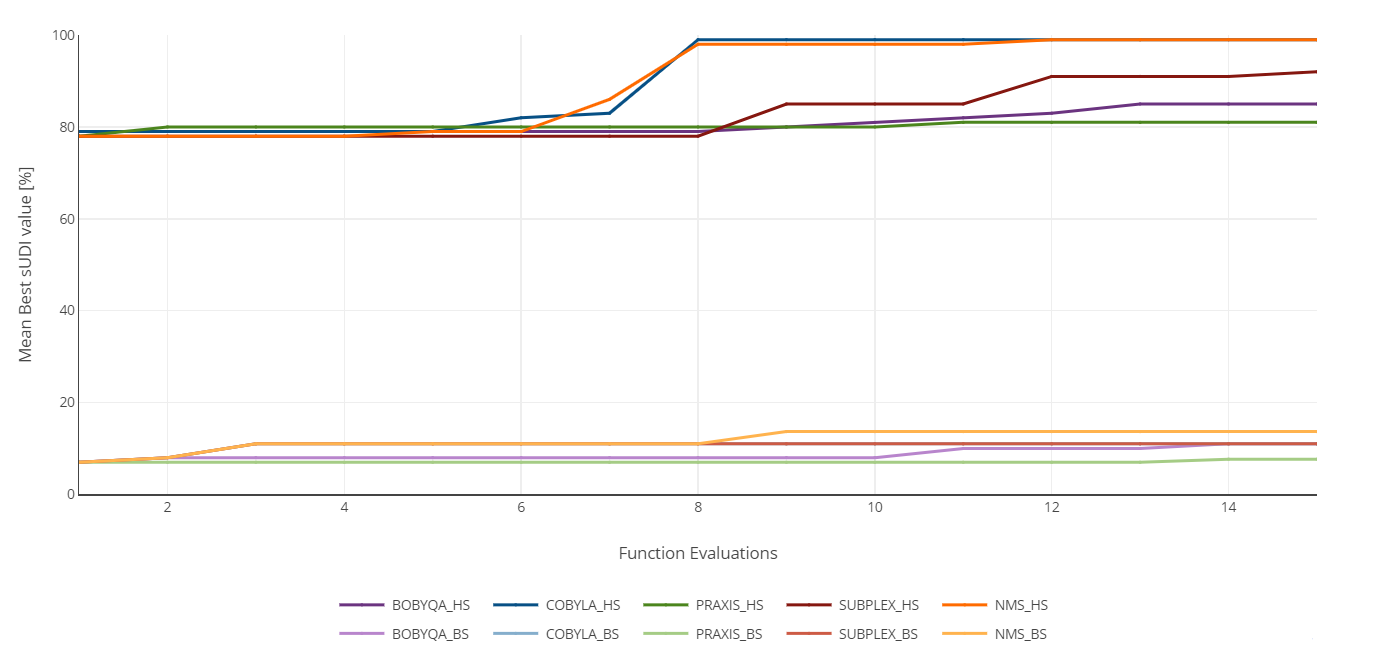
\includegraphics[width=\textwidth]{Images/Evaluation/Ericeira_results_ph2.PNG}
	\caption[Ericeira Solarium: Average best results of daylight conditions (measured in \ac{sUDI}) per local algorithm]{Ericeira Solarium: Average best results of daylight conditions (measured in \ac{sUDI} per local algorithm, as a function of the number of function evaluations. Algorithms suffixed with HS are given an initial solution with an sUDI value of 78\%, whilst algorithms suffixed with BS are given an initial solution with an sUDI value of 7\%.}
	\label{fig:phase2results}
\end{figure}


% #############################################################################
\subsection{Space Frame Optimization}

Besides the real-world case study, we addressed a \ac{MOO} problem \cite{Belem2019MOO}. Given the interest of architects in performing structural analysis \cite{Cichocka2017SURVEY}, we created an artificial case study, whose goal was to optimize both the structural behavior and an ad-hoc measure of irregularity of an arc-shaped space frame. To instil irregularities in this space frame, we introduced three attractors to cause a deformation in the shape of the truss, each of which is defined in terms of the fixed-radius cylindrical coordinates in the arc-shaped space frame. To measure the goals for each design variant, we used (1) the Robot analysis tool to measure the maximum displacement and (2) the sum of the Euclidean distances to measure the total distance between the attractors. To produce an interesting case study, we set to minimize both objective, thus promoting the conflict between these objectives. On the one hand, compressing all the attractors in the same coordinates will increase the maximum displacement of the space frame and, therefore, reduce the structural behavior of the design. On the other hand,  to improve the maximum displacement the attractors should be scattered in along the space frame. However, this implies larger distances among the three attractors. \Cref{fig:spaceframe} illustrates three examples of the space frame structure. 

\begin{figure}[htbp]
	\centering
	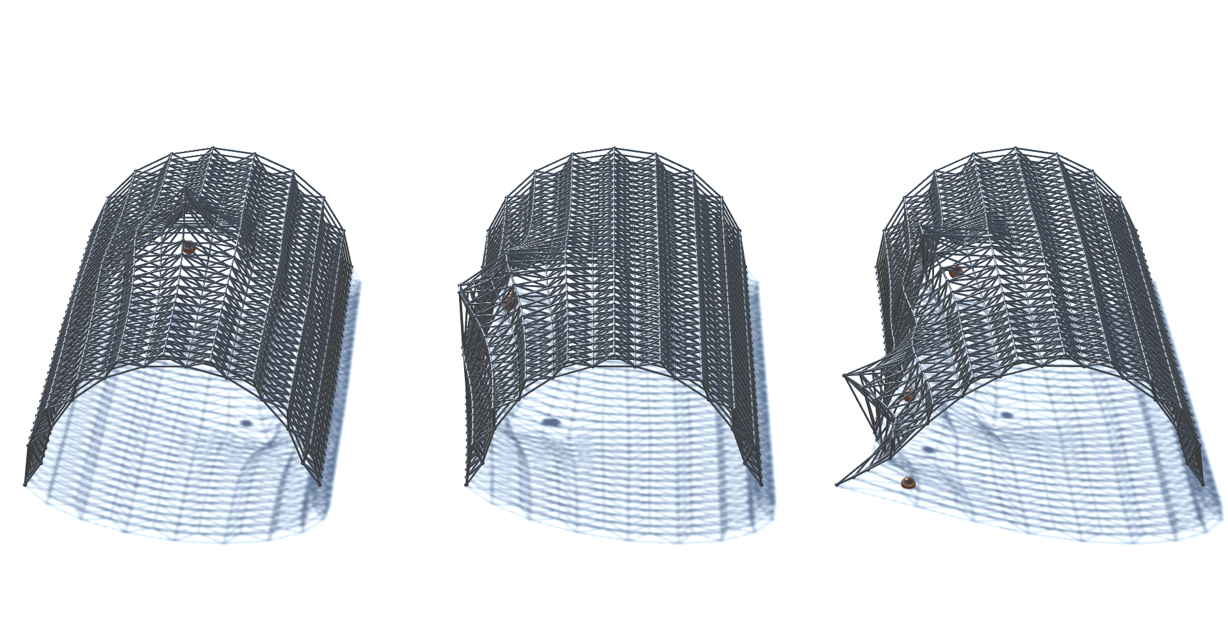
\includegraphics[width=1\textwidth]{Images/Evaluation/truss-kat.png}
	\caption[Space Frame: Representation of three space frame design variants]{Space Frame: Representation of three design variations of the arc-shaped space frame, with copper balls representing the three attractors.}
	\label{fig:spaceframe}
\end{figure}

To optimize the space frame, we decided to test 10 metaheuristics and 9 model-based algorithms. On the one hand, each metaheuristic ran comprised a total of 15 individuals/particles per iteration, which were evolved for 15 iterations. On the other hand, model-based algorithms derived 100 initial samples using the Latin Hypercube Sampling, which were then used to create the initial approximation to the expensive evaluation function, upon which another 125 evaluations were made. Overall, every algorithm was limited to a total of 225 costly function evaluations. 

\todo{Melhorar...}
The evaluation of these algorithms consisted in the computation of different unary performance indicators (discussed in ~\cref{ssec:performance}), some of which required a reference set to be compared with. Ideally, this reference set would represent the true pareto front in order to obtain a more fine measure of each algorithm's performance, however this is not possible. For this reason, and to better approximate the true Pareto front, we determined for each run, each composed of 4275 candidate solutions, the set of optimal solutions, which we named the combined Pareto front. Afterwards, in an attempt to measure the average performance of each algorithm, we computed the performance indicators for each run using each run's combined Pareto front as a reference set. Although this does not represent an accurate approximation of the true Pareto front, we aim at providing an idea of each algorithm's performance on average. To successfully overcome this limitation, the algorithms should run for thousands of iterations instead of a few hundreds. However, time is a limiting factor in \ac{BPO} problems and, therefore, we restrained to measure the average performance of each algorithm, when no other information is known.

\Cref{table:spaceframe,table:spaceframestd} show the results for the algorithms' performance averaged over the three runs. These tables discriminate the algorithms by class and subclass. Since we are addressing a \ac{MOO} problem, the result of each algorithm is measured in terms of unary performance indicators. These indicators provide information about the three different relevant aspects of a Pareto front: (1) the cardinality, measured by \ac{ONVG}, \ac{ONVGR}, and \ac{ER}; (2) the diversity, measured with Spacing, Spread, and Maximum Spread; and (3) accuracy/convergence, measured with \ac{MPFE} and \ac{GD}. Moreover, we further use two indicators that provide a general view over the three aspects, which are the \ac{HV} and the \ac{IGD}. To simplify the performance comparison among the different algorithms, we restrained the set of indicators to the unary ones. 
% 1 - Two set coverage não ia dar medidas relevantes porque raramente as diferentes frentes se tocam. 
% 2 - Epsilon indicators poderia ser interessante, mas não foi testada a implementação
% 3 - R-metrics requer funções de utilidade que não temos e que requer alguma sensibilidade em relação ao problema...

% The overall cardinality of each combined Pareto front is 14, 24, and 19, respectively.
When considering the cardinality aspect, metaheuristics algorithms seem to retrieve the most nondominated solutions within each run, whereas the model-based algorithms seem to retrieve the least. In fact, among the model-based algorithms, the algorithms exploring random search strategies, i.e., which are suffixed with ``\textit{Random}'', yield less nondominated solutions, which may derive from a poor exploration of the solution space. This tendency is further translated when we compare the optimal solutions ratio between each algorithm and the combined Pareto fronts. The \ac{ONVGR} column of \cref{table:spaceframe} presents this ratio. On average, \textit{PAES} doubles the number of solutions found by each combined Pareto front, whereas model-based algorithms, including GPR+Random and the \acp{MLP} algorithms struggled to find a set of optimal solutions with at least half of the size of the combined Pareto fronts. 

%http://papers.cumincad.org/data/works/att/caadria2018\_278.pdf
\begin{table}[htbp]
	\centering
	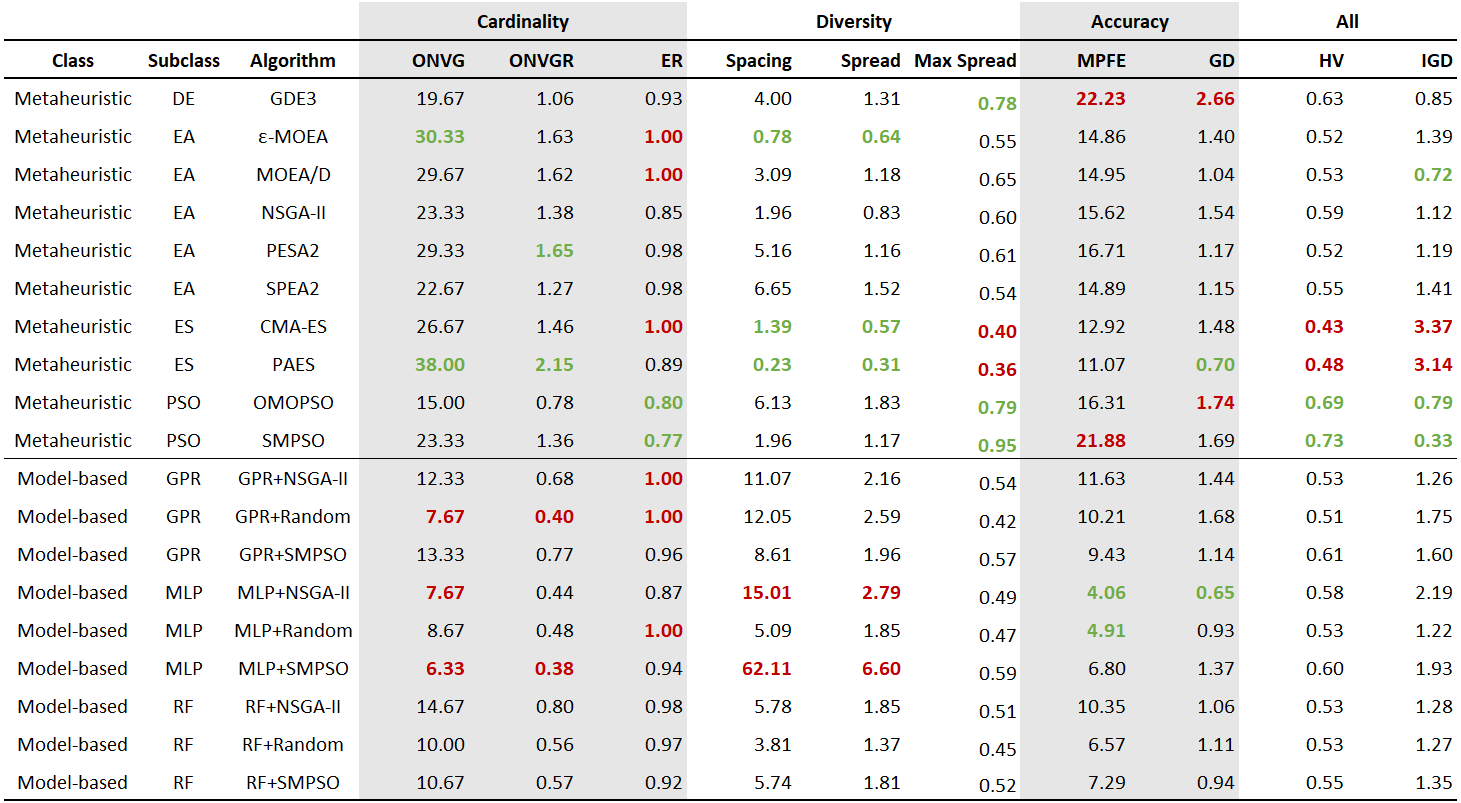
\includegraphics[width=\textwidth]{Images/Evaluation/caadria/Results_Mean_20190413.PNG}
	\caption[Space Frame: Mean performance values of the algorithms' results]{Space Frame: Comparison of the algorithms' mean results for the bi-objective space frame optimization problem. Results are averaged over 3 runs, each with 225 evaluations.}
	\label{table:spaceframe}
\end{table}

While \ac{ONVG} and \ac{ONVGR} indicators provide an intuition abouth the richness of each algorithm's results, many of the identified solutions might not be truly optimal, i.e., despite being the optimal solutions from all the solutions evaluated by a specific algorithm, they do not belong to the true Pareto front (or in this case to the combined Pareto front of the corresponding run). To this end, \ac{ER} is used to measure the percentage of false-optimal solutions for each algorithm. In this case, it becomes clear that even though PAES twice as many nondominated solutions as the combined fronts, most of them are not truly nondominated. Moreover, none of the solutions found by the $\epsilon$-MOEA, MOEA/D, and CMA-ES metaheuristics algorithms, and by the GPR+NSGAII, GPR+Random, and MLP+Random model-based algorithms were not able to find true optimal solution in any of the 3 runs. On the other hand, the \ac{PSO}-based metaheuristics algorithms, SMPSO and OMOPSO, exhibit, on average, the less false-optimal solutions, having found at least one true optimal solution in each run (\cref{appendix:appendixB}).

The diversity aspect consists in the analysis of the distribution of the nondominated solutions. Both Spacing and Spread indicators measure the uniformity of the set of optimal solutions retrieved by each algorithm, regardless of the combined Pareto Front. The former uses the Manhattan distance, whereas the latter uses the Euclidean distances between two consecutive solutions. Considering these indicators, the two \ac{ES}-based metaheuristic algorithms, \textit{PAES} and \textit{CMA-ES}, and one \ac{EA}-based metaheuristic algorithm, \textit{$\epsilon$-MOEA}, achieved the most uniform Pareto Fronts. Conversely, model-based algorithms seem to yield more irregular Pareto fronts, namely, \textit{MLP+NSGA-II} and \textit{MLP+SMPSO} achieved the worst values of both Spacing and Spread indicators. Nevertheless, these indicators only provide an idea of the regularity of the distribution of the solutions. Ideally, these indicators would imply that the there is a good coverage of the Pareto Front. However, the majority of the algorithms that scored the best in the Spacing and Spread indicators achieve such values because the majority of the optimal solutions lie within the same small region in the solution space, thus yielding an uniform distribution. Additionally, the number of solutions also contributes indirectly to these indicators, since these algorithms count the distances between consecutives optimal solutions and the weight each outlier has in smaller or larger sets can greatly influence the final result.

Besides a uniform distribution, a good Pareto front should cover, when applicable, larger extents of the objective space, in order to provide more relevant trade-offs. The Maximum Spread indicator (referred to as Max Spread in \cref{table:spaceframe, table:spaceframestd}) measures the extent of each Pareto front. On average, \textit{SMPSO}, \textit{GDE3}, and \textit{OMOPSO} are able to explore wider extents of the solution space. Observing \cref{table:spaceframe}, we observe that, on average, \textit{SMPSO}, \textit{GDE3}, and \textit{OMOPSO} were able to cover the objective space better. Constrastingly, the \ac{ES}-based algorithms were the worst algorithms in this aspect, having explored smaller regions of the objective space. Regarding model-based algorithms, it is possible to observe that the ones based on \textit{SMPSO} were able to explore broader regions of the objective space than the ones based on \ac{NSGA-II} or \textit{Random} strategies. 

\begin{table}[htbp]
	\centering
	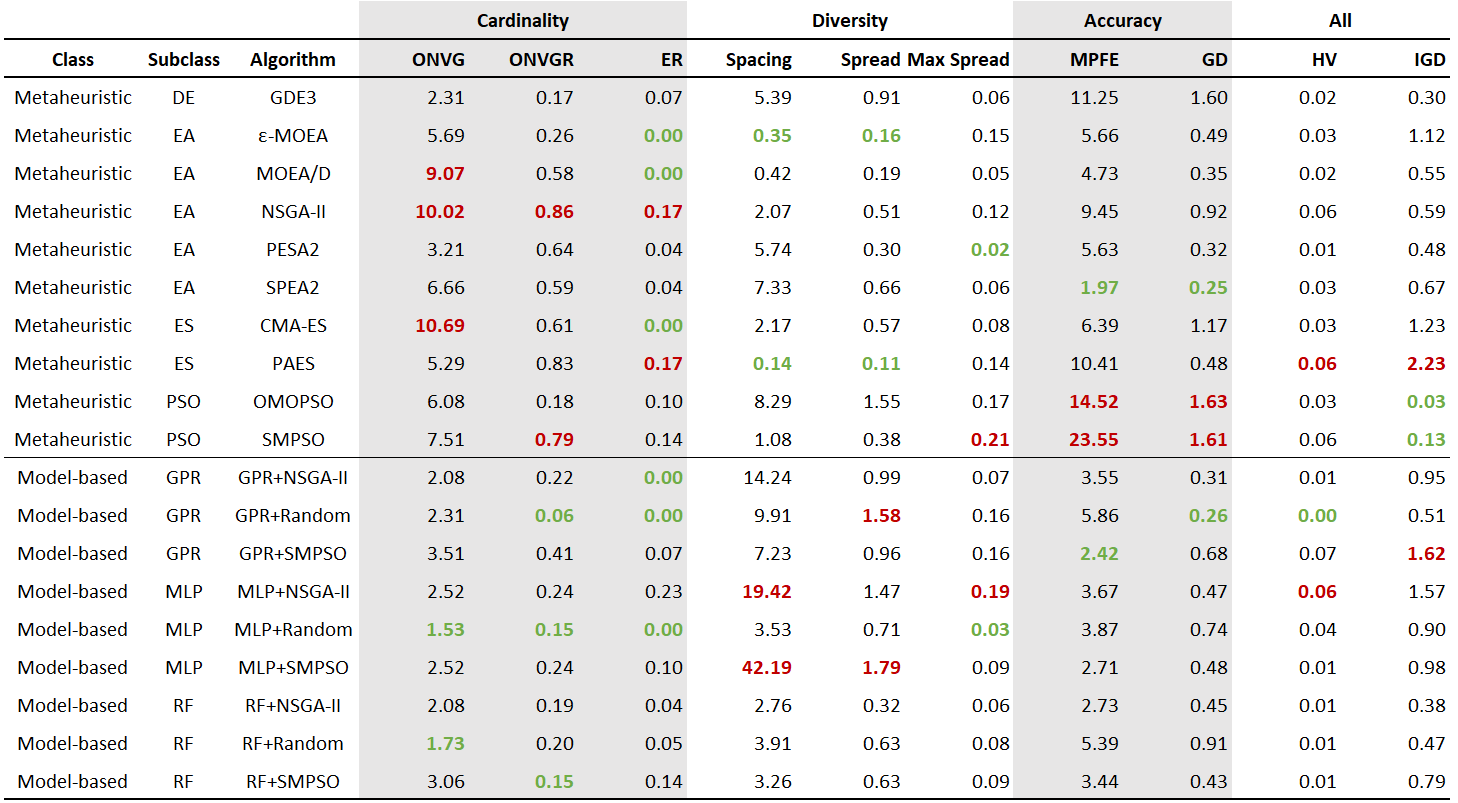
\includegraphics[width=\textwidth]{Images/Evaluation/caadria/Results_Std_20190413.PNG}
	\caption[Space Frame: Standard deviation values of the algorithms' results]{Space Frame: Comparison of the standard deviation for each algorithm's results for the bi-objective space frame optimization problem. Results are averaged over 3 runs, each with 225 evaluations.}
	\label{table:spaceframestd}
\end{table}

The accuracy aspect measures how close the solutions are from the true Pareto front. As previously mentioned, in this dissertation, we consider the true Pareto front to be the result of the best solutions found in each run. This decision aims at measuring the average performance of each algorithm when obtaining information about the real true Pareto front is unfeasible. In this case study, we used two accuracy indicators, namely the \ac{MPFE} and the \ac{GD}. On average, when considering \ac{MPFE}, every model-based algorithm retrieved Pareto fronts, whose \ac{MPFE} values were always better than the ones obtained by any metaheuristic. In particular, \textit{MLP+NSGA-II} and \textit{MLP+Random} have the smallest maximum error which means that all the points are at most at that distance from an optimal solution. Furthermore, it seems that the algorithms exploring a larger extent of the objective space, i.e., which higher values of Max Spread, have worse \ac{MPFE} values. This can be explained due to the lack of information about the true Pareto front, which is only approximated by the best solutions found in that run instead of the true Pareto front, or even the combination of all runs. 

Notwithstanding the fact that \ac{MPFE} provides an estimate of the maximum error of the algorithms' results, it does not provide a real measure of how close the results are to the optimal front, or, in this case, the combined Pareto front. To this end, we use the \ac{GD} indicator, which measures the average approximation of the results of an algorithm to the closest solutions in the combined Pareto front. \Cref{table:spaceframe} shows that, on average, \textit{MLP+NSGA-II} and \textit{PAES} present the best convergence towards the combined Pareto front, and that \textit{GDE3} and \textit{OMOPSO} present the worst convergence. This can be explained by the number of the nondominated solutions retrieved by each algorithm, as well as the creation of clusters of optimal solutions nearby the combined Pareto front. It is possible to observe that the Pareto fronts discovered by \textit{PAES} and \textit{MOEA/D} present several agglomerations of optimal solutions nearby the combined Pareto front (see \cref{sec:spaceframeoptimizationextra} \todo{WRONG REF}). In general, other model-based algorithms also present reasonable scores, like the \textit{MLP+Random} or all the \ac{RF}-based algorithms even surpassing many metaheuristics algorithm, including \textit{CMA-ES}, \textit{$\epsilon$-MOEA}, \textit{\ac{NSGA-II}}, and \textit{\ac{SPEA2}}, thus suggesting better approximations.

In the end, we also used the \ac{IGD} and the \ac{HV} indicators, as they provide a general view over the quality of a Pareto front with regards to all three aspects simultaneously. Regarding \ac{HV}, the best performing algorithms were the \ac{PSO}-based algorithms, \textit{SMPSO} and \textit{OMOPSO}, followed by \textit{GDE3}. Surprisingly, the \ac{PSO} model-based algorithms also present a good performance, when compared to other metaheuristics and even other model-based algorithms that explore \textit{random} or \ac{EA} strategies during the search for optimal solutions. On the other hand, the worse performing algorithms were the \ac{ES}-based metaheuristics, \textit{CMA-ES} and \textit{PAES}, followed by \textit{GPR+Random}. Finally, comparing different algorithms regarding \ac{IGD}, the \ac{PSO}-based metaheuristic algorithms still yield the best results, whilst \ac{ES}-based metaheuristic algorithms retrieve the worst. However, \textit{MOEA/D} unexpectedly reveals itself as the third most performing algorithm when considering the \ac{IGD} indicator. Although this seems odd, this value can be explained by the difference in the scales of both axis.

\begin{figure}[htbp]
	\centering
	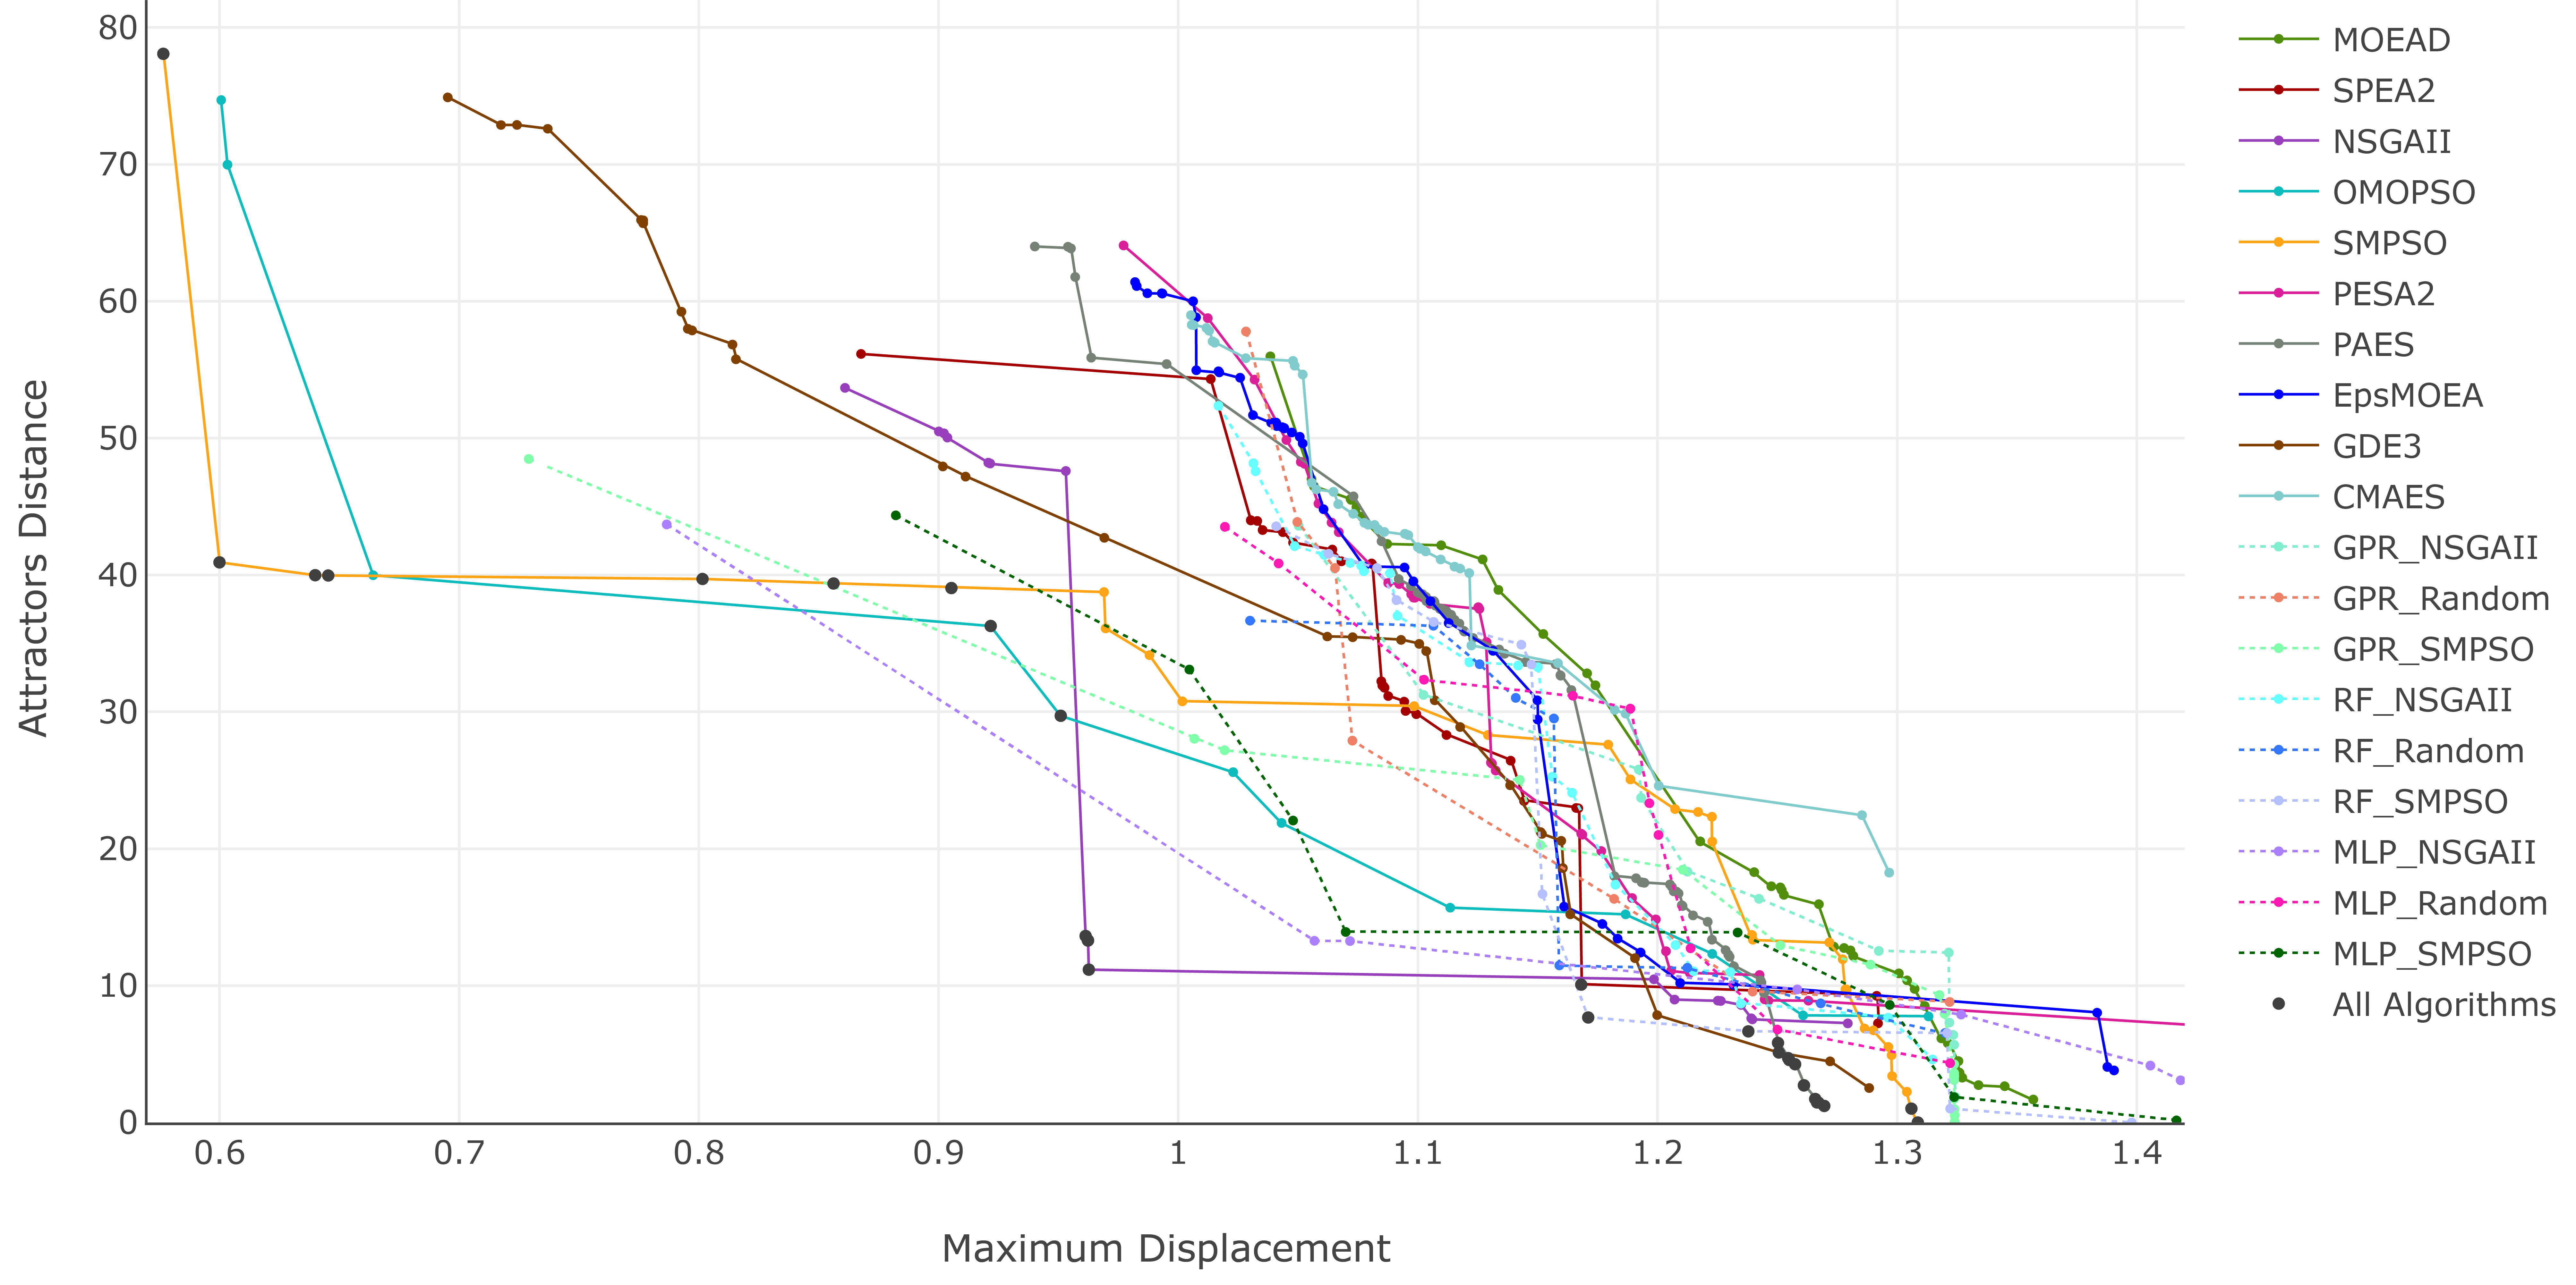
\includegraphics[width=\textwidth]{Images/Evaluation/caadria/All_Algorithms_all_runs-2019-04-13_600dpi.png}
	\caption[Space Frame: Overview over the algorithms' Pareto fronts]{Space Frame: Overview over the algorithms' Pareto fronts for the bi-objective space frame optimization problem. These fronts are obtained by combining the values of the 3 runs for each algorithm. The combined Pareto front is formed by finding the nondominated solutions from all the evaluated solutions.}
	\label{fig:allruns}
\end{figure}

Overall, no single algorithm was able to outperform the others in terms of the three aspects: cardinality, diversity, and cardinality. Nevertheless, the \ac{PSO}-based metaheuristics algorithms, \textit{OMOPSO} and \textit{SMPSO}, exhibited the overall best performance. Moreover, even though none of the model-based algorithms was able to surpass the \textit{SMPSO} and \textit{OMOPSO}, the model-based algorithms that use \textit{SMPSO} also exhibited a reasonable performance, better than several well-known metaheuristics, including \textit{$\epsilon$-MOEA}, \textit{MOEA/D}, \textit{CMA-ES}, and \textit{\ac{SPEA2}}. \Cref{fig:allruns} presents a combined view of all the algorithms for every run, where it is possible to visualize the extent of \ac{PSO}-based algorithms and the high density region to which several \acp{EA} and \acp{ES} algorithms converged.

\subsection{Black Pavilion: Skylights Optimization}

- INVOLVE OPTIMIZAÇÃO LUMINICA E DE CUSTO.


\subsection{Other cases...}

- Adaptive Façades: Thermal